\section{The need for fine-granularity streams (existing techniques)}
Here we argue that streaming by bit planes or streaming by levels result in sub-optimal PSNR (figure \ref{fig:psnr_traditional_vs_by_norm_viscosity}a)

\begin{figure}[t]
	\centering
	\subcaptionbox{without skip leading zeros}
	{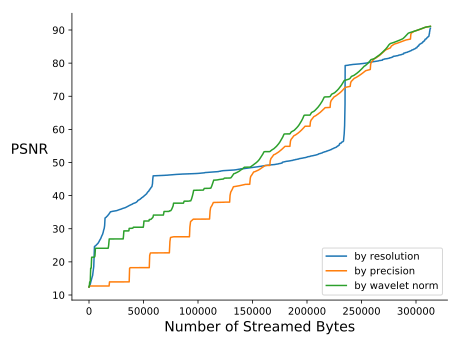
\includegraphics[width=0.4\linewidth]{resources/rmse-miranda-viscosity.png}}
	\subcaptionbox{with skip leading zeros}
	{\includegraphics[width=0.4\linewidth]{resources/rmse-miranda-viscosity_slz.png}}
	\caption {PSNR comparison between three streams: by bit-plane, by level, and by wavelet norm}
	\label{fig:psnr_traditional_vs_by_norm_viscosity}
\end{figure}

When compression is used, it avoids streaming the leading zero bits of the wavelet coefficients (figure \ref{fig:psnr_traditional_vs_by_norm_viscosity}b).

In the supplement materials, we show the same plot for the following datasets:
Datasets:
\begin{enumerate}
  \item Miranda viscosity (smooth and uniform)
  \item Kingsnake (noisy and sparse)
  \item Magnetic (tiny narrow lines)
  \item Euler 2D (sharp front)
  \item Enzo u (wide range)
\end{enumerate}

The reader may ask: if I already have a good, practical PSNR stream (the data-independent, by bit plane, skip leading zeros), why do I need other streams? Here we show that for isocontour extraction, and for histogram computation, we are better off with other streams.
  
\begin{enumerate}
  \item Figure 3: isocontour error for the same data set (Figure \ref{fig:by_bit_plane_isocontour})
  \begin{enumerate}
    \item Data-dependent stream for isocontour with skip leading zeros
    \item Data-dependent stream for isocontour with skip leading zeros, also with by-bit-plane constraint
  \end{enumerate}
  We also need to show a rendering of the two isocontours for these streams at some low bit rate.
  Figure 4: histogram error for the same data set
  \begin{enumerate}
    \item Data-dependent stream for histogram with skip leading zeros
    \item Data-dependent stream for histogram with skip leading zeros, also with by-bit-plane constraint
\end{enumerate}  
  Here we also show renderings of different histograms corresponding to the different streams at some low bit rate.
\end{enumerate}

\begin{figure}
  \centering
  \includegraphics[width=0.8\linewidth]{resources/isocontour-error-by-bit-plane-viscosity.png}
  \caption {By bit-plane isocontour comparison versus no constraints for viscosity, isoval=-0.005}
  \label{fig:by_bit_plane_isocontour}
\end{figure}
